
\chapter{北京谱仪实验}
\label{chap:bes3}

北京正负电子对撞机~(${\rm BEPC}$)~和相应的探测器北京谱仪~({BES})~于~{1988}~年~{10}~月
在中国科学院高能物理研究所建成。{1994}~年至~{1996}~年间,
对撞机和探测器进行了升级,升级后的对撞机仍称为~BEPC,探测器称为~BESII。升级后的对撞机和探测器的性能均有了很大的改进,取得了一系列在国际高能物理届有重要影响的研究成果,如~$\tau$~轻子质量的精确测量、$2 \sim 5 \gev$~的强子反应截面~(R~值)~的精确测量、粲夸克偶素衰变的系统研究等。2003~年底,国家批准了北京正负电子对撞机重大改造工程。该工程于~2004~年开始动工,2008~年竣工,2009~年通过国家验收并开始收集物理事例。升级后的对撞机和探测器分别称为~BEPCII~和~BESIII。至今为止,BESIII~已收集大量的实验数据,如表~\ref{tab:bes3data}~ 所示,并取得了丰硕的研究成果。

\begin{table}[!htb]
\centering
\small
\setlength{\abovecaptionskip}{0pt}
\setlength{\belowcaptionskip}{5pt}
\caption{BESIII~收集的实验数据简介。}
\begin{tabular}{lcc}
\toprule
数据样本 &  质心系能量~($\gev$) & 积分亮度或事例数 \\ \hline
$\jpsi$~数据 & $3.097$ & $1.3\times10^9$ \\
$\psip$~数据 & $3.686$ & $4.5\times10^8$ \\
    $\psipp$~数据 & $3.773$ & $2.9\,{\rm fb}^{-1}$ \\
    $\tau$~轻子质量扫描数据 & 3.554 & $24\,{\rm pb}^{-1}$ \\
    $XYZ$~数据 & 3.81$\sim$4.6 & $5\,{\rm fb}^{-1}$ \\
    $R$~值和~QCD~数据 & $2\sim3,\ 3.85\sim4.59$ & $0.5\,{\rm fb}^{-1},0.8\,\rm{fb}^{-1}$ \\
\bottomrule
\end{tabular}%
\label{tab:bes3data}
\end{table}

本章主要包括北京正负电子对撞机的简介、北京谱仪的物理目标和探测器结构以及北京谱仪的离线软件系统的介绍。

\section{北京正负电子对撞机}
BEPC~是工作在~$\tau$-粲能区的高亮度、多束团的正负电子对撞机~\cite{BEPCII},
而升级后的~BEPCII~的峰值亮度比它的前身还要高了两个量级。BEPCII~主要由注入器、束流输运线
和储存环构成。注入器是一台长度为~202\,m~的直线加速器,
由电子枪产生的电子以及由电子打靶产生的正电子一起被直线加速器加速后,
经由束流输运线注入到储存环中。储存环是一台环形的加速器,
正负电子束流在环内被累积、加速、储存和对撞。
BEPCII~在原有的储存环隧道的基础上采用双环方案,
使正负电子束流能够在两个彼此独立的储存环中累积、加速,并在对撞点处发生对撞。
双环结构是使束流亮度能够提高两个量级的关键\cite{BESIII-design}。
BEPCII~的主要性能参数可参见表~\ref{tab:BEPCII}。
值得一提的是,$2016$~年,BEPCII~的亮度达到了
$1 \times 10^{33} {\rm cm}^{-2} {\rm s}^{-1}$~的量级,
处于世界的前列。
此外,北京正负电子对撞机还实现了所谓的“一机两用”,
即在同步辐射模式下,可以作为光源以供物理研究。
\begin{table}
    \centering
    \small
    \setlength{\abovecaptionskip}{0pt}
    \setlength{\belowcaptionskip}{5pt}
    \caption{BEPCII的主要设计参数。}%
    \label{tab:BEPCII}
    \begin{tabular}{lc}
        \toprule
        束流能量~$E_{b}\,\gev$        & $1.0\sim2.3$  \\
        设计亮度~($E_{b}=1.89\,\gev$) & $1 \times 10^{33}\,{\rm cm}^{-2}{\rm s}^{-1}$ \\
    高频频率~(MHz)                & $499.8$ \\
    对撞周期~(ns)                 & $8$ \\
    储存环长度~(m)                & $237.53$ \\
    束团数目                      & $93$ \\
    正负电子注入速率~(mA/min)     & $50$ \\
    \bottomrule
\end{tabular}%
\end{table}

\begin{figure}
    \centering
    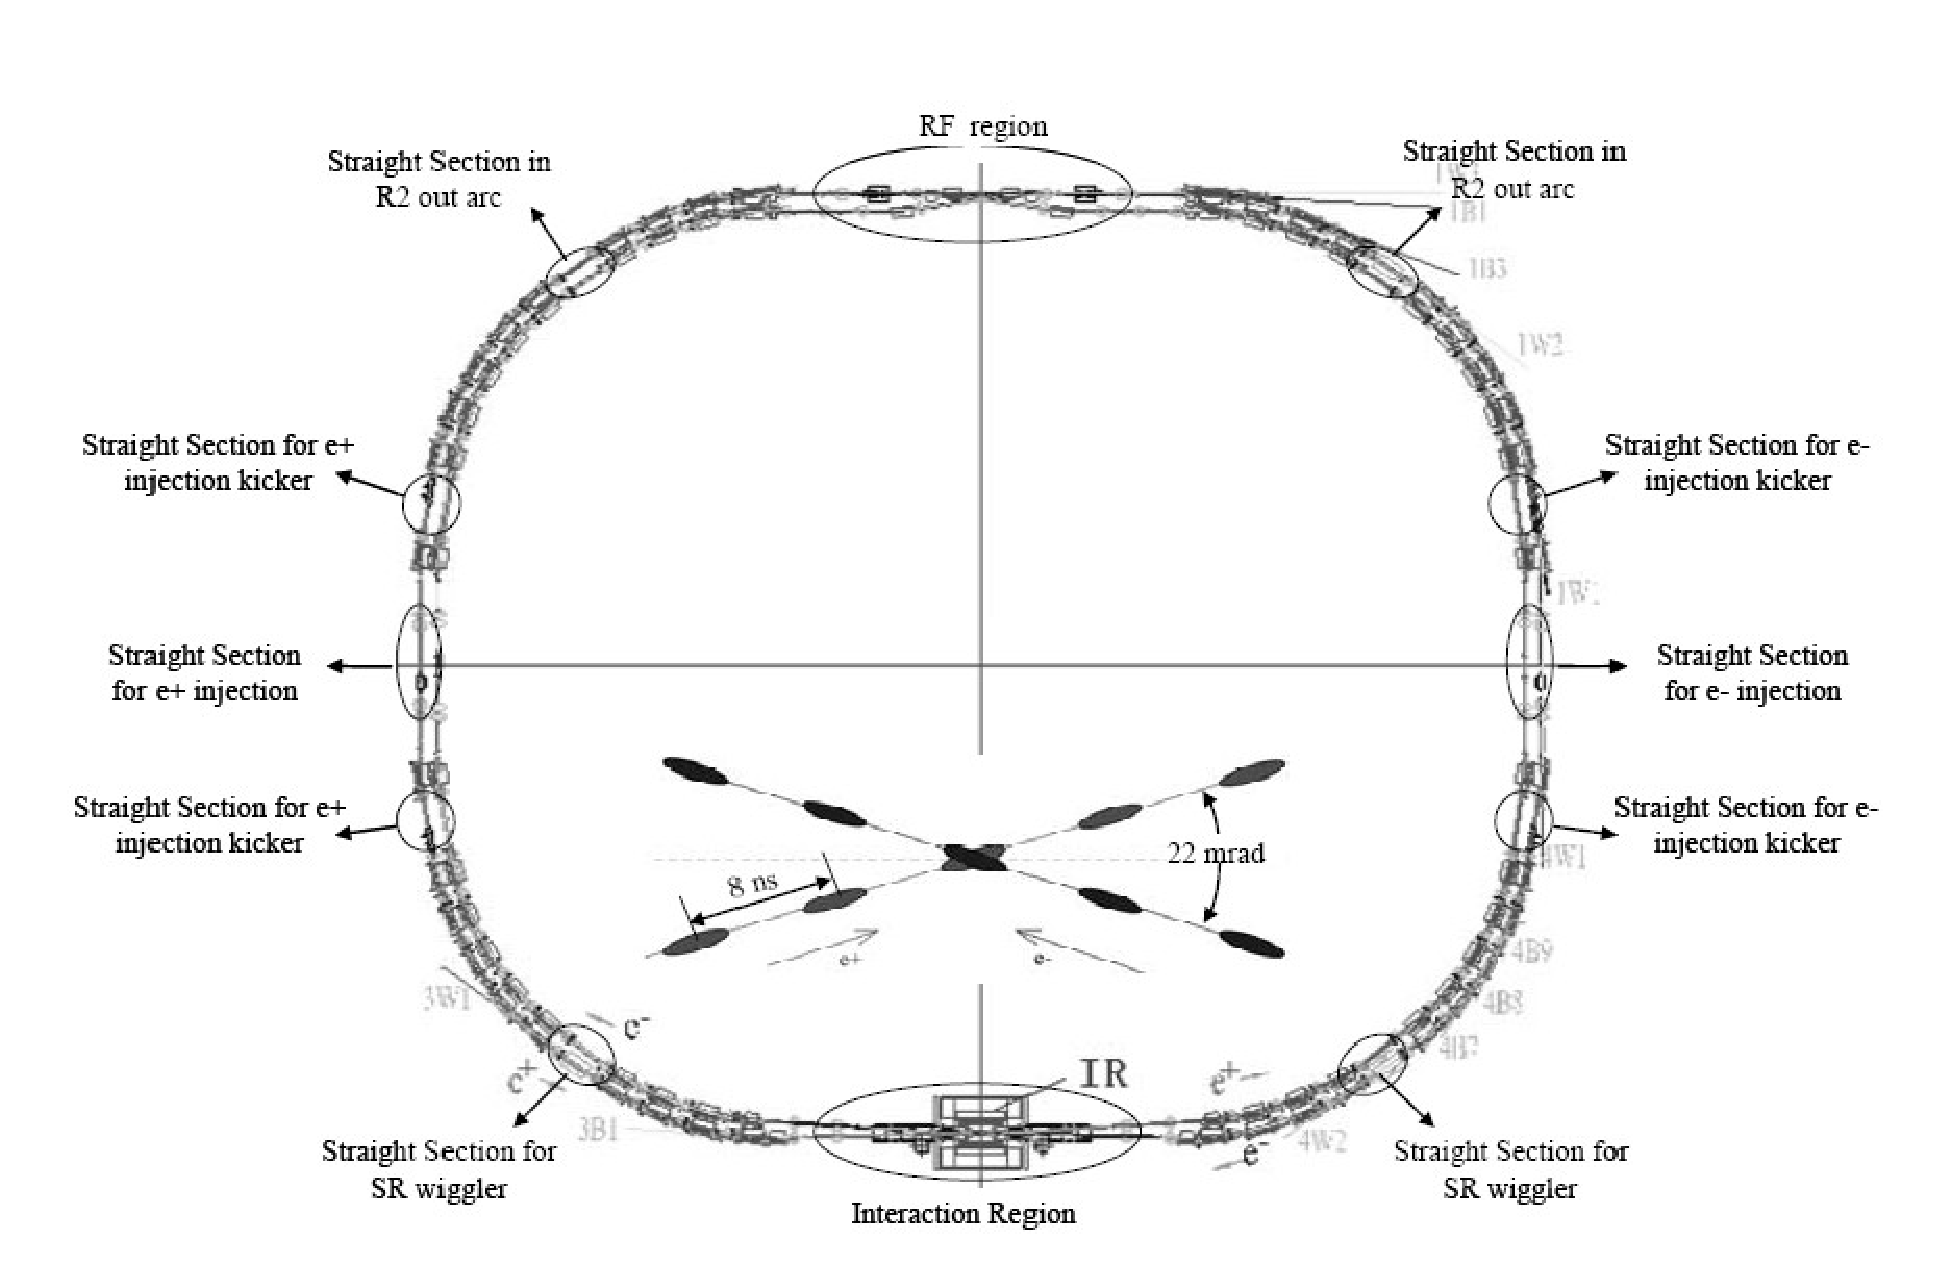
\includegraphics[width=0.8\textwidth]{bes3/BEPCII.eps}
    \caption{BEPCII俯视图。}%
    \label{fig:BEPCII}
\end{figure}

\section{北京谱仪}
BESIII~是运行在~BEPCII~上的工作于~$\tau$-粲能区的大型通用探测器~\cite{bes3},
其主要物理目标包括 $\tau$-粲能区的电、弱、强相互作用的研究以及新物理的寻找等
~\cite{bes3phys}。在收集了高统计量的数据的基础上,
BESIII~是用来精确检验标准模型和寻找新物理的理想场所。

BESIII~可以对电、弱相互作用理论提供精确的检验:通过对~$D$~和~$D_{s}$~介子衰变的精确测量来检验~CKM~(Cabibbo-Kobayashi-Maskawa)~\cite{CKM}~矩阵元的幺正性;通过对~$\tau$~轻子质量的精确测量来对轻子普适性提供更高精度的检验;通过对~$\tau^+\tau^-$~ 近域高精度的截面测量来加深对~$\tau^+\tau^-$~间相互作用的理解;利用~$\lcp\lcm$~阈值上的对撞数据,精确测量~$\lcp$~的各强子衰变以及半轻子衰变的性质。

由于强相互作用在~$\tau$-粲能区的非微扰性,使得目前在该能区的理论计算均具有
很大的不确定性。BESIII~利用~$\tau$-粲能区的数据对~QCD~展开了研究,
其中主要包括:结合高精度的~LQCD~的计算对标准模型的基本参数进行测量,
如强相互作用的耦合常数~$\alpha_{s}$~等;对低能强子谱进行研究,
寻找~QCD~预言的各种包含胶子的态,如胶球等;研究粲偶素的产生和衰变,
对量子色动力学提供精确检验。

BESIII~通过持续高亮度的运行,积累了大量的数据。
因而可以在~BESIII~上进行稀有衰变的寻找,如寻找味道改变中性流~(FCNC)~过程、
轻子数或重子数破坏的过程等。此外在标准模型中~$D^{0}-\bar{D^{0}}$~的混合
以及~$D_{s}$/$D$~衰变中的~$CP$~破坏效应都很小,而一些新物理模型可以加强
这种效应。在~BESIII~上利用高统计量的数据也可以对中性~$D$~介子的混合
及~$CP$~破坏进行寻找。

为了实现以上物理目标,BESIII~探测器需要满足的要求有:
\begin{itemize}
    \item 对光子进行精确测量,具有好的能量分辨、角度分辨以及识别能力;
    \item 对低动量带电径迹进行探测,精确测量其动量和角度信息;
    \item 好的粒子鉴别能力,能够对各种粒子进行区分,如电子、$\mu$~子、
        $\pi$~介子、$K$~介子和质子等;
    \item 好的前端电子学系统、触发系统和数据获取系统,适应~BEPCII~多束团模式
        下的高取数率,减少死时间。
\end{itemize}

根据以上的要求,BESIII~探测器的总体结构如图~\ref{fig:BESIII}~所示,
由内而外依次是主漂移室~(Main Drift Chamber, MDC)、
飞行时间计数器(Time-of-Flight, TOF)、
电磁量能器~(Electro-Magnetic Calorimeter, EMC)、
超导磁体~(Superconductor Magnet)~和~$\mu$~子计数器~(Muon Counter, MUC)。
BESIII探测器的主要性能参数~\cite{bes3}~可见表~\ref{tab:bes3p}。

\begin{figure}
 \centering
 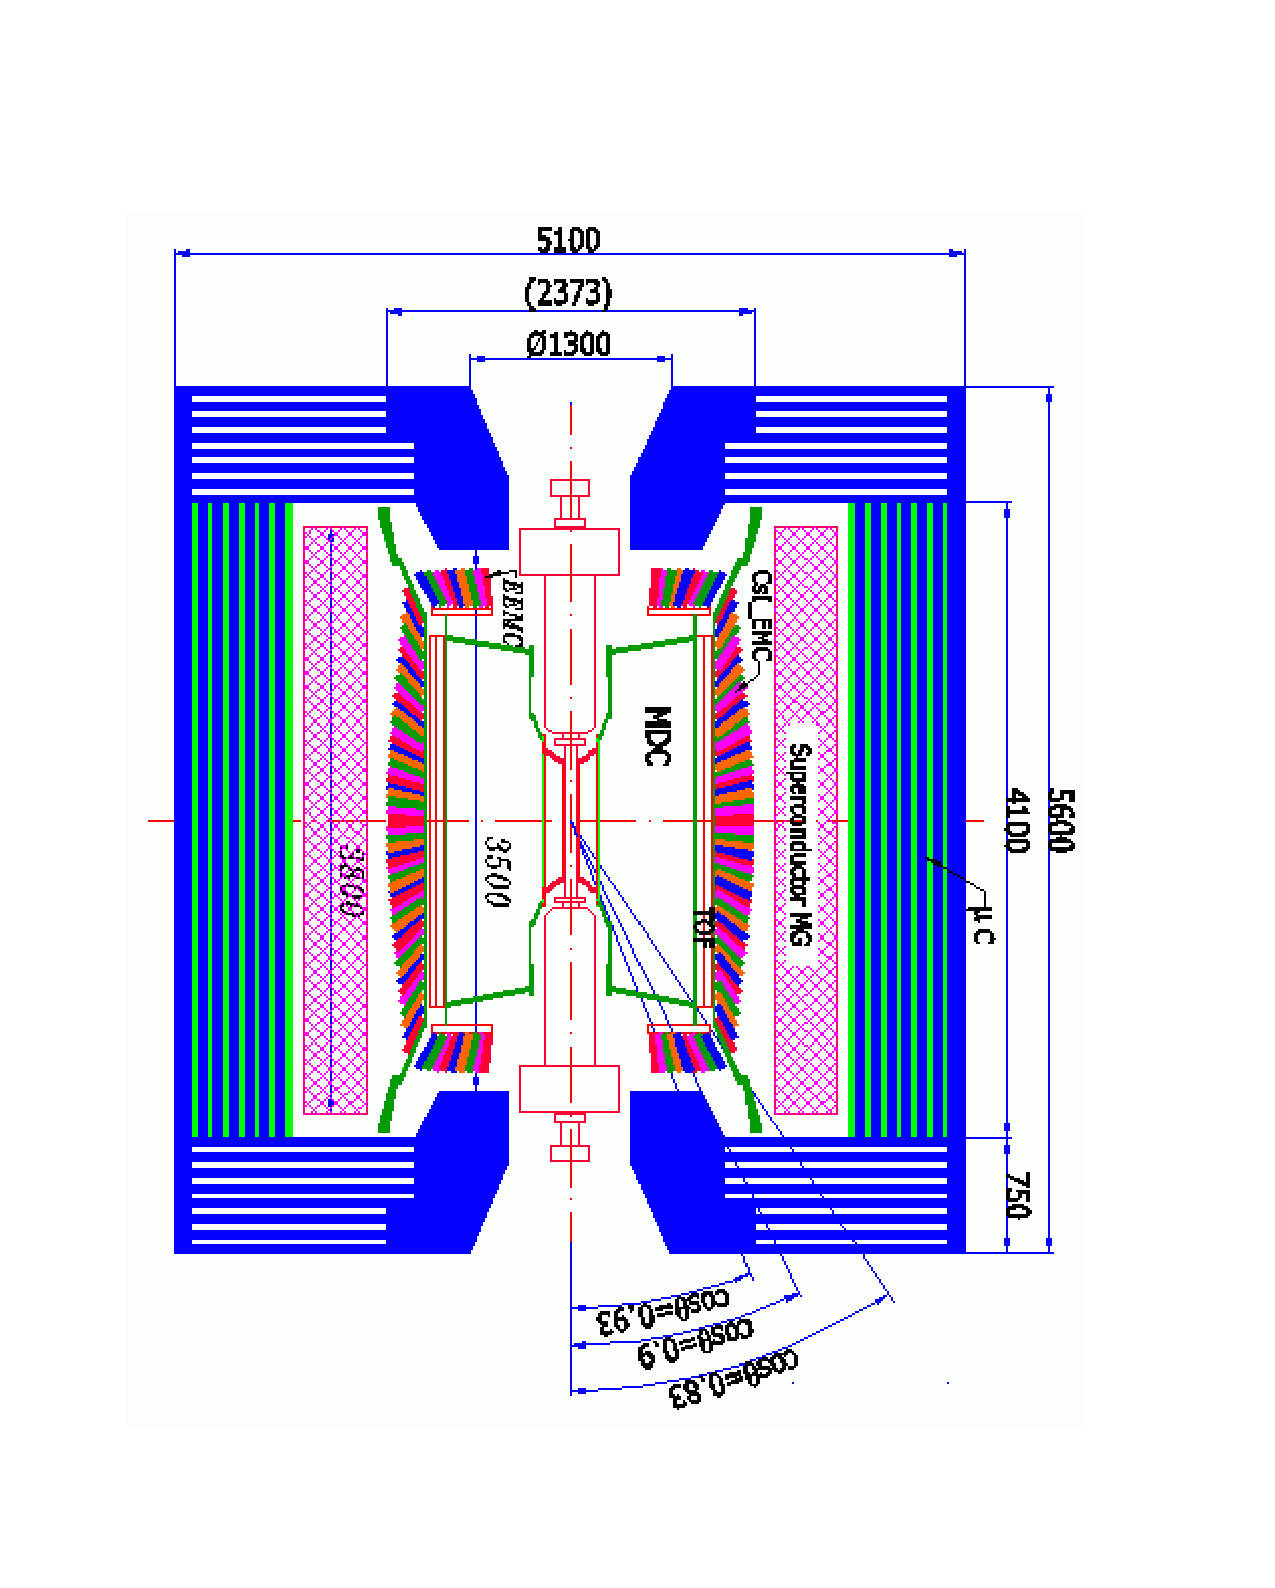
\includegraphics[angle=90,width=0.8\textwidth]{bes3/bes_view.eps}
 \caption{BESIII探测器的结构侧视图。}
 \label{fig:BESIII}
\end{figure}

\begin{table}
\centering
\footnotesize
\caption{BESIII主要性能参数。}
\begin{tabular}{ll}
\toprule
子系统                         & 主要性能参数 \\
\midrule
\multirow{3}* {主漂移室}       & $\sigma_{xy}$=130\ $\mu$m            \\
                               & $\Delta P$/{\it{P}}=0.5\ \% @1.0\ GeV     \\
                               & $\sigma_{dE/dx}$=6\ \%              \\
\midrule
\multirow{2}* {飞行时间计数器} &  $\sigma_{t}$= 100\ ps 桶部  \\
                               &  $\sigma_{t}$= 110\ ps 端盖  \\
\midrule
\multirow{2}* {电磁量能器}     &  $\sigma_{E}$/{\it{E}}=2.5\ \% @1.0\ GeV  \\
                               &  $\sigma_{\phi z}$=0.6\ cm  @1.0\ GeV  \\
\midrule
$\mu$ 子计数器                 &   9\ 层   \\
磁场强度                       &   1.0\ T \\
\bottomrule
\end{tabular}
\label{tab:bes3p}
\end{table}

\subsection{束流管}
束流管是储存环的一部分,它位于探测器的中心,分为中心束流管和外延束流管。其中中心束流管采用具有低原子序数且强度足够高的铍管,用来减小物质层的厚度,以减少多次散射对径迹动量分辨的影响。中心铍管采用了双层结构,中间为液态冷却系统,用来带走由粒子损失、同步辐射、次级粒子散射以及高频腔高次模产生的热量。两侧的外沿束流管由铜管或镀铜铝管制成,以减少因同步辐射产生的散射光子。

\subsection{主漂移室}
主漂移室是~BESIII~的最重要的子探测器,是一个与束流管相邻的圆柱形漂移室,
它的主要任务有:
1)~精确测量带电径迹的动量和方向;
2)~为带电径迹的粒子鉴别提供~$dE/dx$~信息;
3)~为带电径迹的一级硬件触发提供信号。
主漂移室采用了低质量材料,以及小单元的结构。考虑到对撞区的束流本底会
严重影响主漂移室的工作寿命,同时为了方便地安装束流管等部件,
主漂移室被设计成内室和外室两个部分。主漂移室沿径向一共有~43~层信号丝,
其中内室有~8~层,外室有~35~层。每~4~ 个信号丝层称为一个超层。
为了测量带电粒子的~$z$~坐标,内室的~2~个超层被设计为斜丝层,
其中第一个超层的斜丝相对于轴作负~$\phi$~方向的倾角排列,
第二个超层的斜丝为正~$\phi$~向的倾角排列。

BESIII~采用了强度为~1.0\,Tesla~的超导磁场。通过对带电粒子在磁场中的
飞行轨迹进行测量,从而计算出其动量大小和方向。
带电粒子在主漂移室内的工作气体中飞行时会发生电离,产生电子-离子对。
其中电子在电场的作用下会向信号丝漂移,正离子则向场丝漂移。
电子在漂移的过程中会发生雪崩放大,倍增后的电子被信号丝收集而产生电流,
这称为信号丝的一次着火。根据带电粒子在各层信号丝中留下的一连串的着火信息,
可以对其飞行轨迹进行测量。一般来说,飞行轨迹上的着火点越多,
动量的测量精度也就相应越高。 此外,根据~Bethe-Bloch~公式,
不同的带电粒子在同一工作气体中飞过单位路程所损失的能量~($dE/dx$)~是不同的,
如图~\ref{fig:dedx}~所示。通过对信号丝收集的电荷总量可以计算出粒子
的~$dE/dx$~信息,从而对粒子的类型进行鉴别。

带电粒子在主漂移室中飞行的过程中,会与探测器的物质层作用而发生多次库仑散射,
这将会对动量的测量精度造成影响。出于以上考虑,
主漂移室的工作气体使用氦气与丙烷的混合气体,场丝使用低原子序数的铝丝,
内室和外室的端面板也采用铝制材料,内、外桶采用炭纤维材料。
主漂移室的漂移单元采用小单元设计,如图~\ref{fig:mdc_danyuan_XT}~所示,
在每个小单元之中,信号丝位于中心,四周是接近方格分布的~8~或~9~根场丝。
主漂移室采用这种结构的优点是:
1)~减小粒子的漂移距离,缩短漂移时间,提供快速的触发信息,适合高计数率下的工作;
2)~减小电子扩散的贡献,获得更好的空间分辨;
3)~减少信号丝上的累积电荷,增长工作寿命;
4)~单元排列紧密,减少测量的死区,使~$dE/dx$~具有更好的分辨;
5)~ 具有多个测量单元,可以在有限的空间内提供更多的测量次数。
但是这种小单元结构也有一些不足:
1)~有些单元内电场分布不均匀,导致漂移距离和漂移时间的关系变复杂;
2)~单元边缘的电场会发生畸变,导致较强的边缘效应。
在一个小单元内,漂移距离~$X$~和漂移时间~$T$~的关系
可参见图~\ref{fig:mdc_danyuan_XT}。

内室的端面板被设计成小台阶形状,这种设计减小了端面板和内外室连接部件的变形。
外室的端面板包含了台阶部分和斜面部分。其中台阶部分的设计是为了满足
主漂移室的立体覆盖角达到~0.93\%$\times4\pi$,以及保证与束流管相连的
加速器的~Micro-$\beta$~聚焦磁铁的安放和电缆的引出有足够的空间。
斜面部分的设计,则是为了减小端面板在丝张力下的变形。
\begin{figure}
\begin{center}
 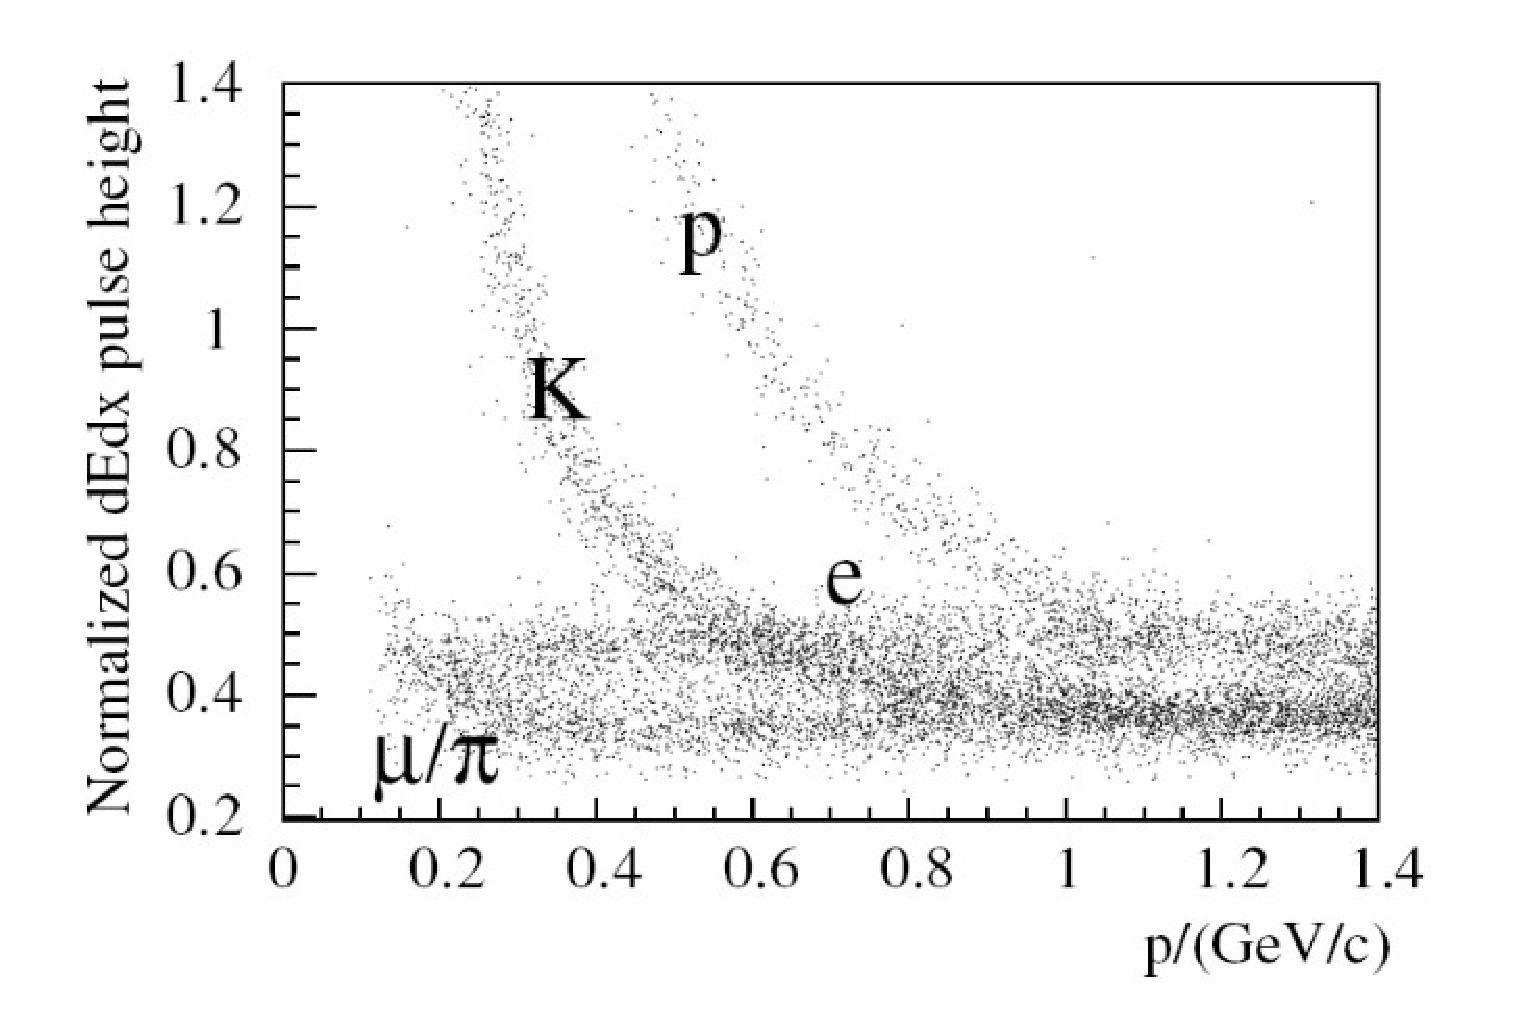
\includegraphics[width=0.55\textwidth]{bes3/dedx.eps}
 \caption{带电粒子的归一化脉冲高度~($dE/dx$)~随动量分布的散点图。}
 \label{fig:dedx}
 \end{center}
\end{figure}

\begin{figure}
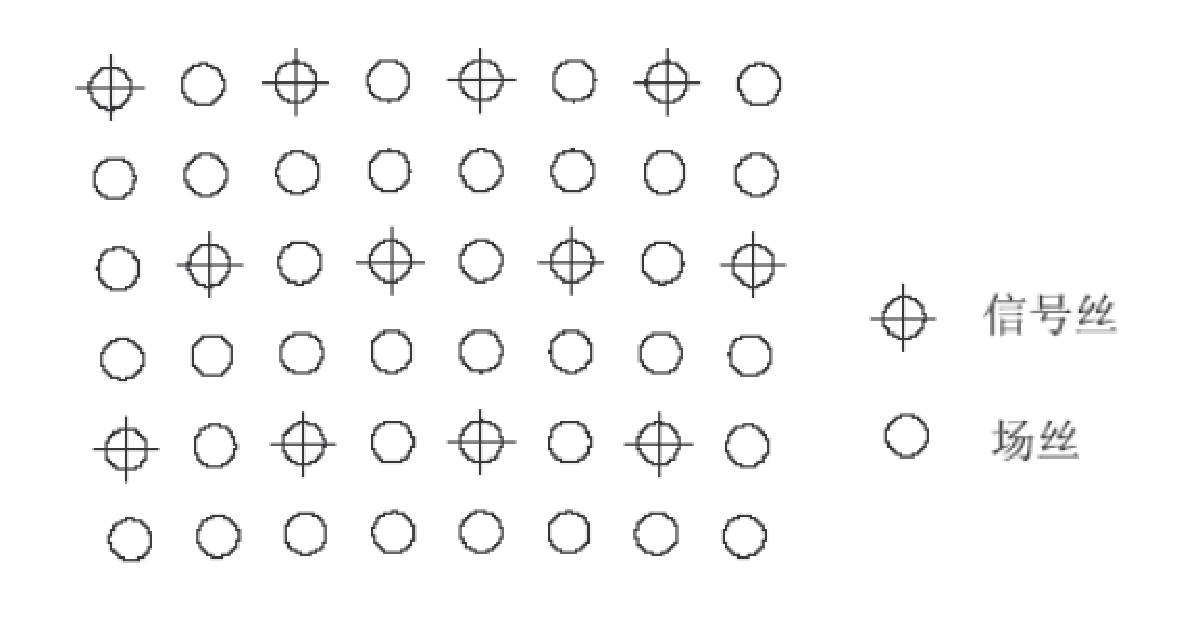
\includegraphics[width=0.5\textwidth]{bes3/mdc_danyuan.eps}
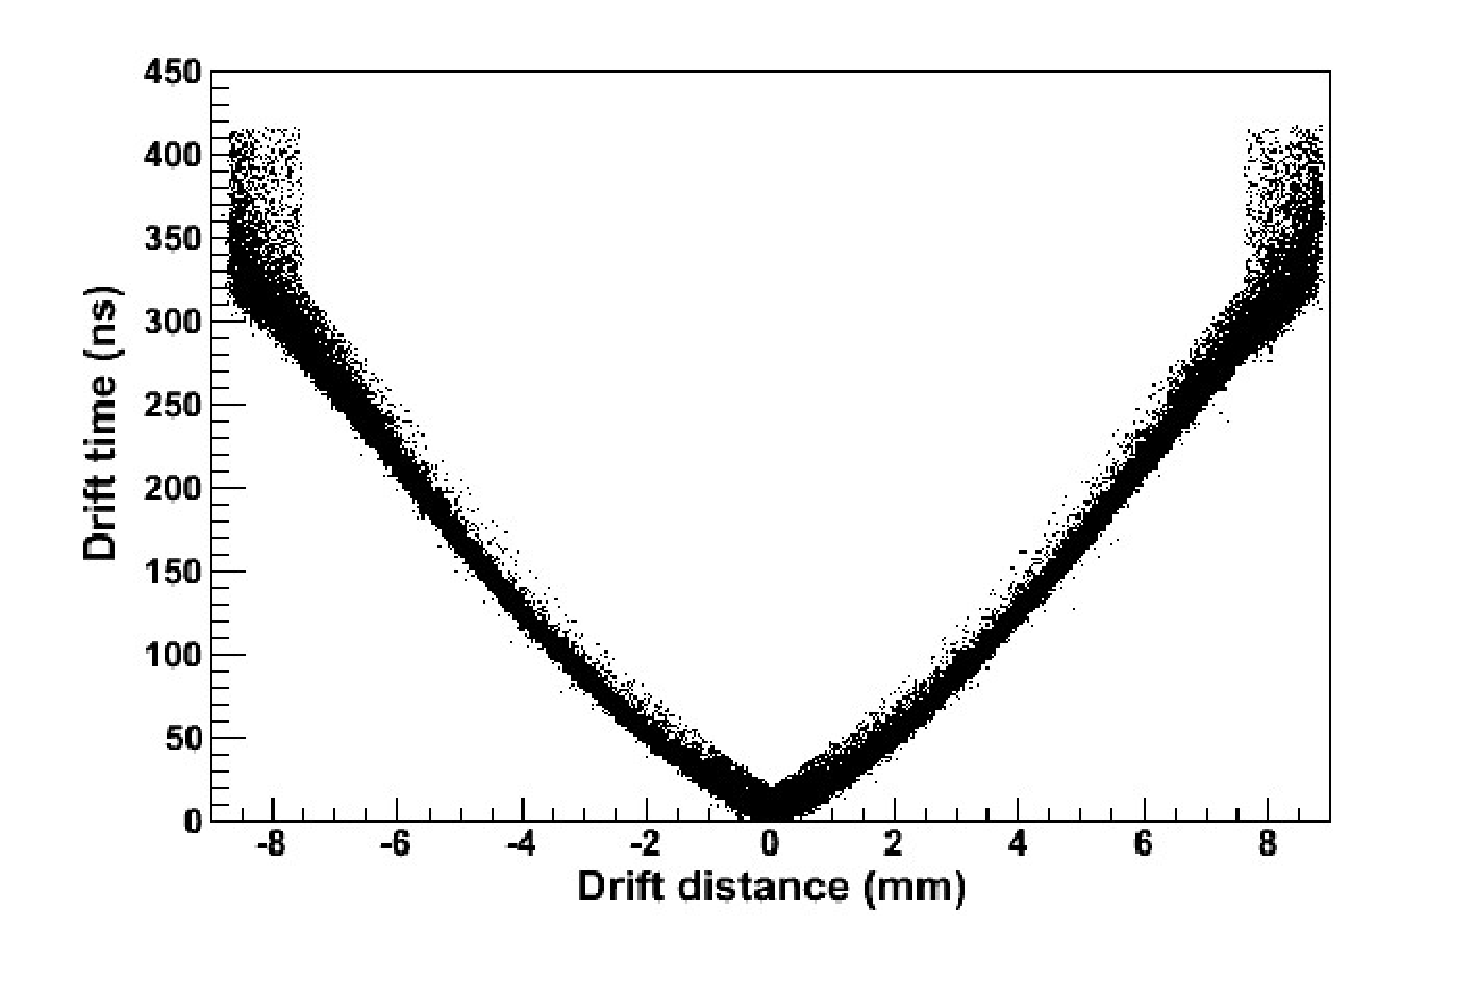
\includegraphics[width=0.4\textwidth]{bes3/X_T.eps}
\caption{漂移室的单元结构示意图(左)。漂移距离~$X$~和漂移时间~$T$~的关系(右)。}
\label{fig:mdc_danyuan_XT}
\end{figure}

\subsection{飞行时间计数器}
\label{subsection:tof}
飞行时间计数器的主要作用对飞行时间进行精确测量,并结合主漂移室测得的
粒子动量信息对粒子的种类进行鉴别。同时,飞行时间计数器还参与了初级触
发判选,利用不同探测器输出信号之间的时间信息排除来自宇宙线的本底。

飞行时间计数器位于主漂移室的外部,同样也分为桶部和端盖两部分。
其中桶部的接收立体角为~$82\%\times 4\pi$, 端盖的接收立体角
为~$10\%\times 4\pi$,$\cos\theta$~在~0.85$\sim$0.95~之间。
整个飞行时间计数器基本覆盖了主漂移室的接收度。飞行时间计数
器采用了塑料闪烁体作为探测元件,两端和光电倍增管连接在一起。
桶部采用了双层闪烁体结构,每个闪烁体具有两端读出,端盖采用
了单层结构,分为东西两部分,单端读出。桶部固定在主漂移室上,
端盖固定在电磁量能器上。桶部的设计分辨为~80$\sim$90\,ps, 
端盖的设计分辨为~80\,ps。在~$2\sigma$~鉴别能力的要求下,桶
部对于~$K/\pi$~的分辨可达到~0.9\,GeV/c。

飞行时间探测器主要由闪烁体、光导、光电倍增管和电子学四部分组成,
在~2015~年还在端盖部分安装了多隙阻性板探测器~(MRPC)。当高能带电
粒子穿过时,会与闪烁体发生作用,从而使闪烁体中的原子或分子电离而
损失能量。受激发的原子或分子在退激发过程中会发射光子,光子在闪烁
体内传播并由光阴极收集而发生光电效应,在光阴极上打出光电子,光电
子通过光电倍增管放大并被记录。

通过测量粒子的飞行时间,结合主漂移室测得动量和径迹信息,飞行时间
计数器可按照如下原理对粒子种类进行鉴别。
一个带电粒子的质量~$m$~和速度~($c \beta$)~应满足如下公式
\begin{equation}
\beta c  = \frac{L}{t_{tof}},\ m^2 = p^2 \times \frac{1-\beta^2} {\beta^2c^2},
\label{eq:mp}
\end{equation}
其中~$c$~表示光速,$L$~为飞行距离,$t_{tof}$~为粒子的飞行
时间,$p$~是粒子的动量大小。
从公式~(\ref{eq:mp})~我们可以看出粒子的飞行时间与其质量相关,
我们据此可以判断其粒子类型。

我们假定粒子的类型为~$i$,然后利用以下公式计算出其预期飞行时间:
\begin{equation}
t^i_{exp} = L  \sqrt{(\frac{m_i}{p})^2 + 1 },
\end{equation}
然后定义预期的飞行时间~$t^i_{exp}$~和与测得的飞行时间~$t_{tof}$~的
偏差为~$\chi_{TOF}^i$,$\chi_{TOF}^i$~的绝对值越小,粒子为~$i$~的概率越大。

\subsection{电磁量能器}
\label{subsection:emc}
电磁量能器是采用了~CsI~(T1)~晶体制成,而且同样由桶部和端盖两部分组成。
其桶部的内半径为~94\,cm,内长~275\,cm;端盖内半径为~50\,cm,距离对撞
点~Z=$\pm$138\,cm。
桶部共有~44~圈,每圈~120~块晶体。除第一圈外,对撞中心处~$\theta$~向的
左右两部分的晶体均指向距对撞中心~$\pm5$\,cm~的点,每层晶体在~$\phi$~向
相对于中心线有~$1.5\,^{\circ}$~的偏移。
端盖量能器由半圆环组成,在径向共有~6~层晶体结构,每层晶体均指向距对撞中
心~$\pm$10\,cm~的点。

电磁量能器主要用途是精确测量光子或带电粒子产生的电磁簇射,
确定光子的能量和位置信息,并提供中性径迹事例的触发。其工作
原理是:入射光子在物质原子核的库仑场作用下转化成正负电子对,
所产生的正负电子对又进一步发生级联韧致辐射和光子电子对转化。
直到所产生的的光子的能量低于光子转换成电子对的阈值能量时,
簇射过程停止。正负电子对可以激发出晶体能带中的电子--空穴对,
电子--空穴对复合后发出的光被硅光二极管吸收。通过硅光二极管收
集到的光的能量,可以测得到最初的入射粒子能量。

由于韧致辐射的功率与粒子质量的平方成反比,对于~$\gamma$~和
电子而言,在量能器中的辐射长度很短,几乎沉积了所有能量。而
对于其它带电粒子,则辐射长度较长,它们大多只在量能器中沉积
一部分的能量。因此可以利用带电径迹在量能器中的能量沉积与主
漂移室测得的径迹动量的比值~($E/p$)~来把电子和其他粒子鉴别开来。

\subsection{超导磁体}
超导磁体系统的主要用途是为主漂移室提供高强度的均匀稳定的轴向磁场,
用来使带电粒子发生偏转。它由超导线圈、直线电源、真空系统、低温系统
以及磁测系统组成,是BESIII的关键部件之一。磁感应强度的大小有以下考虑:
一方面较高的磁感应强度可以提高粒子动量的分辨,但另一方面过高的磁场也
会对低动量的径迹造成测量的困难。综合以上考虑,超导磁体系统采用由纯铝
为稳定体的~NiTi/Cu~合金缠绕而成的超导磁铁,由液氦作冷却剂,
并使用轭铁~(即~$\mu$~子鉴别器的吸收体)~ 提供磁场回路。超导磁体系统为
漂移室提供了约~1.0\,T~左右的轴向磁场,均匀度为~5\,\%,磁场的测量精度
可达到~0.1\,\%。

\subsection{$\mu$~子鉴别器}
$\mu$~子鉴别器~($\mu$ Chamber)~位于~BESIII~探测器的最外层,包括
由阻性板室~(RPC)~组成的~$\mu$~子鉴别器以及有夹层的轭铁组成的强子
吸收体,工作气体为~$\rm Ar/C_{2}H_{2}F_{4}/iC_{4}H_{10}(50/42/8)$
~混合气。其主要功能是鉴别反应末态中的~$\mu$~子,通过对多层击中点的
位置进行测量来确定粒子的飞行轨迹,再与内层探测器测量的径迹相匹配,
从而鉴别出~$\mu$~子,尤其是区分~$\mu$子~和~$\pi$~介子。

\subsection{触发判选系统}
BEPCII~采用的是多束团、高流强的对撞模式,这种模式极大程度地提高
了对撞亮度,但同时也给~BESIII~探测器带来了很高的本底,从而给后续
的电子学系统、触发判选系统、在线数据获取系统带来了挑战。其中触发
判选系统是快速实时的事例选择和控制系统,该系统需要把~BESIII~收集
的事例率压缩到在线数据获取系统可以接受的程度,并尽可能减少好事例的丢失。

BEPCII~的多个束团间的时间间隔一般为~8\,ns。触发判选系统无法在两次
对撞之间完成一次判选,我们要求触发和电子学系统使用流水线~(Pipe-Line)~
的方式对数据进行缓存与挑选。前端电子学可以缓存一段时间~(6.4\,$\mu$s)~
内的数据,触发判选系统需要在这段时间内完成初级硬件触发,给出触发信号~L1。
没有通过硬件触发的信息将被覆盖或丢弃。

\subsection{数据获取系统}
BESIII~的在线数据获取系统是基于前端电子学系统和触发判选系统的硬件系统,
它由读出系统、在线系统、慢控制系统、校准系统及其它服务系统组成。

数据获取系统的主要用途是收集经过初级触发判选的事例数据,
通过两级计算机的预处理和高速网络传输,将分布在各读出机箱中
的事例数据迅速汇集到在线计算机系统上,然后对事例进行包装和过滤,
组装成完整有效的事例,最终将事例数据标记并记录到永久的存储介质上。
数据获取系统使用了先进的计算机和网络技术,并采用了多级并行的处理方案;
为了从前端电子学系统中快速读出大量数据并尽可能减少系统的死时间,
大量采用了多级数据缓冲技术、并行处理技术、VME~总线高速读出技术及网络传输技术。

\section{离线软件系统}
BESIII~的离线软件系统~(BesIII Offline Software System, BOSS)~由主框架系统、
数据刻度系统、事例重建系统、事例模拟系统、实用软件包系统以及用户分析软件包
组成。其主要用途是对实验数据和蒙特卡洛~(Monte Carlo, MC)~\,\cite{mcsim}~
模拟数据进行处理,并对多种工具库和文件库进行管理。

\subsection{离线软件框架}
BOSS~是基于Gaudi框架,使用~C++~语言和面向对象的技术进行开发的,
它为数据刻度、事例重建、蒙特卡洛模拟及物理分析提供了统一的平台。
BOSS~框架结构以瞬态数据库~(Transient Data)~为核心;
对数据的存储和处理相对独立;提供了标准的用户程序嵌入点;
模块之间的操作通过标准的接口进行;对宿存~(Persistency)~数据和
瞬态数据进行独立管理;模块的开发遵循尽可能重用的原则。
BOSS~框架的主要组成部分为:算法模块~(Algorithm),应用
管理器模块~(Application Manager),瞬态数据库模块~(Transient Data Store),
服务模块~(Service)和转换器模块~(Converters)~等。

\subsection{探测器模拟系统}
蒙特卡洛方法是用来处理随机过程的一种有效方法。在高能物理实验中,通常要靠蒙特卡洛方法估计某个物理过程的探测效率。所以通过蒙特卡洛模拟产生的过程和要尽可能与真实过程一致。在~BESIII~上,这一过程由~(BESIII
Object Oriented Simulation Tool, BOOST)~来完成。BOOST~\cite{BOOST}~是基于高能物理实验中广泛应用的~Geant4~\cite{Ablikim:2009aa}~来开发的面向对象的框架系统,它包括物理事例的产生子、物质与几何结构的描述、磁场的描述、粒子与物质的相互作用、探测器的响应、真实化信息、数据输出和用户界面等部分。事例产生子以~HepEvt~的格式来产生物理事例,然后作为输入提供给~Geant4,接着由~Geant4~来构造探测器并模拟粒子在物质中的相互作用,同时记录下粒子在探测器中的响应信息。模拟系统采用基于~XML~(eXtensible Markup Language)~的统一几何描述标识语言--GDML~(Geometry Description Markup Language)~来构造~BESIII~各个子探测器的物质和几何结构。探测器的响应是独立于~Geant4~的,它利用粒子的击中信息来确定探测器的输出信号,这个过程也称为数字化过程~(Digitization)。探测器的击中信息在经过数字化后得到原始数据~(raw data),同时在模拟阶段也需要记录下模拟时粒子的真实信息~(MC truth)~以供重建和分析时使用。我们通过后期调试~(MC tuning)~ 来减小蒙特卡洛模拟与真实数据的细微差异,蒙特卡洛模拟的好坏直接影响了物理分析的精度。

事例产生子模拟了各种物理过程,根据反应机制和微分截面来生成物理事例,
并计算出初末态所有粒子的四动量信息。BESIII~模拟系统包括了~30~多个产生子,
如均匀相空间的产生子~(howl), $J/\psi\rightarrow\rho\pi$~事例产生
子~(rhopi)、$J/\psi$ 和$\psi(2S)$~单举衰变产生子~(lundcharm)等等。
这些产生子都是在不断完善中的,有时还需要用户根据自己的需求写出相应的产生子。

\subsection{离线重建系统}
BESIII~离线重建系统是~BESIII~离线软件系统的重要组成部分,
它负责利用~BESIII~各个子探测器收集的原始信息来得到末态粒子
的电荷、飞行轨迹、动量大小等感兴趣的物理信息,以供给后续的
物理分析使用。如图~\ref{fig:rec_flow}~所示,BESIII~离线重建
大致包括~MDC、TOF、EMC、MUC~等子探测器的重建和物理事例顶点的
重建~(一般一个~run~对应重建出一个对撞顶点)。其中~MDC~的重建
又包括事例起始时间的重建、MDC~主重建、$dE/dx$~重建、径迹
的Kalman~拟合和径迹的外推等等。
从下图我们可以看出事例起始时间的重建是在整个离线重建系统的最前
沿,直接影响着后续各个系统的重建质量。
\begin{figure}
\begin{center}
 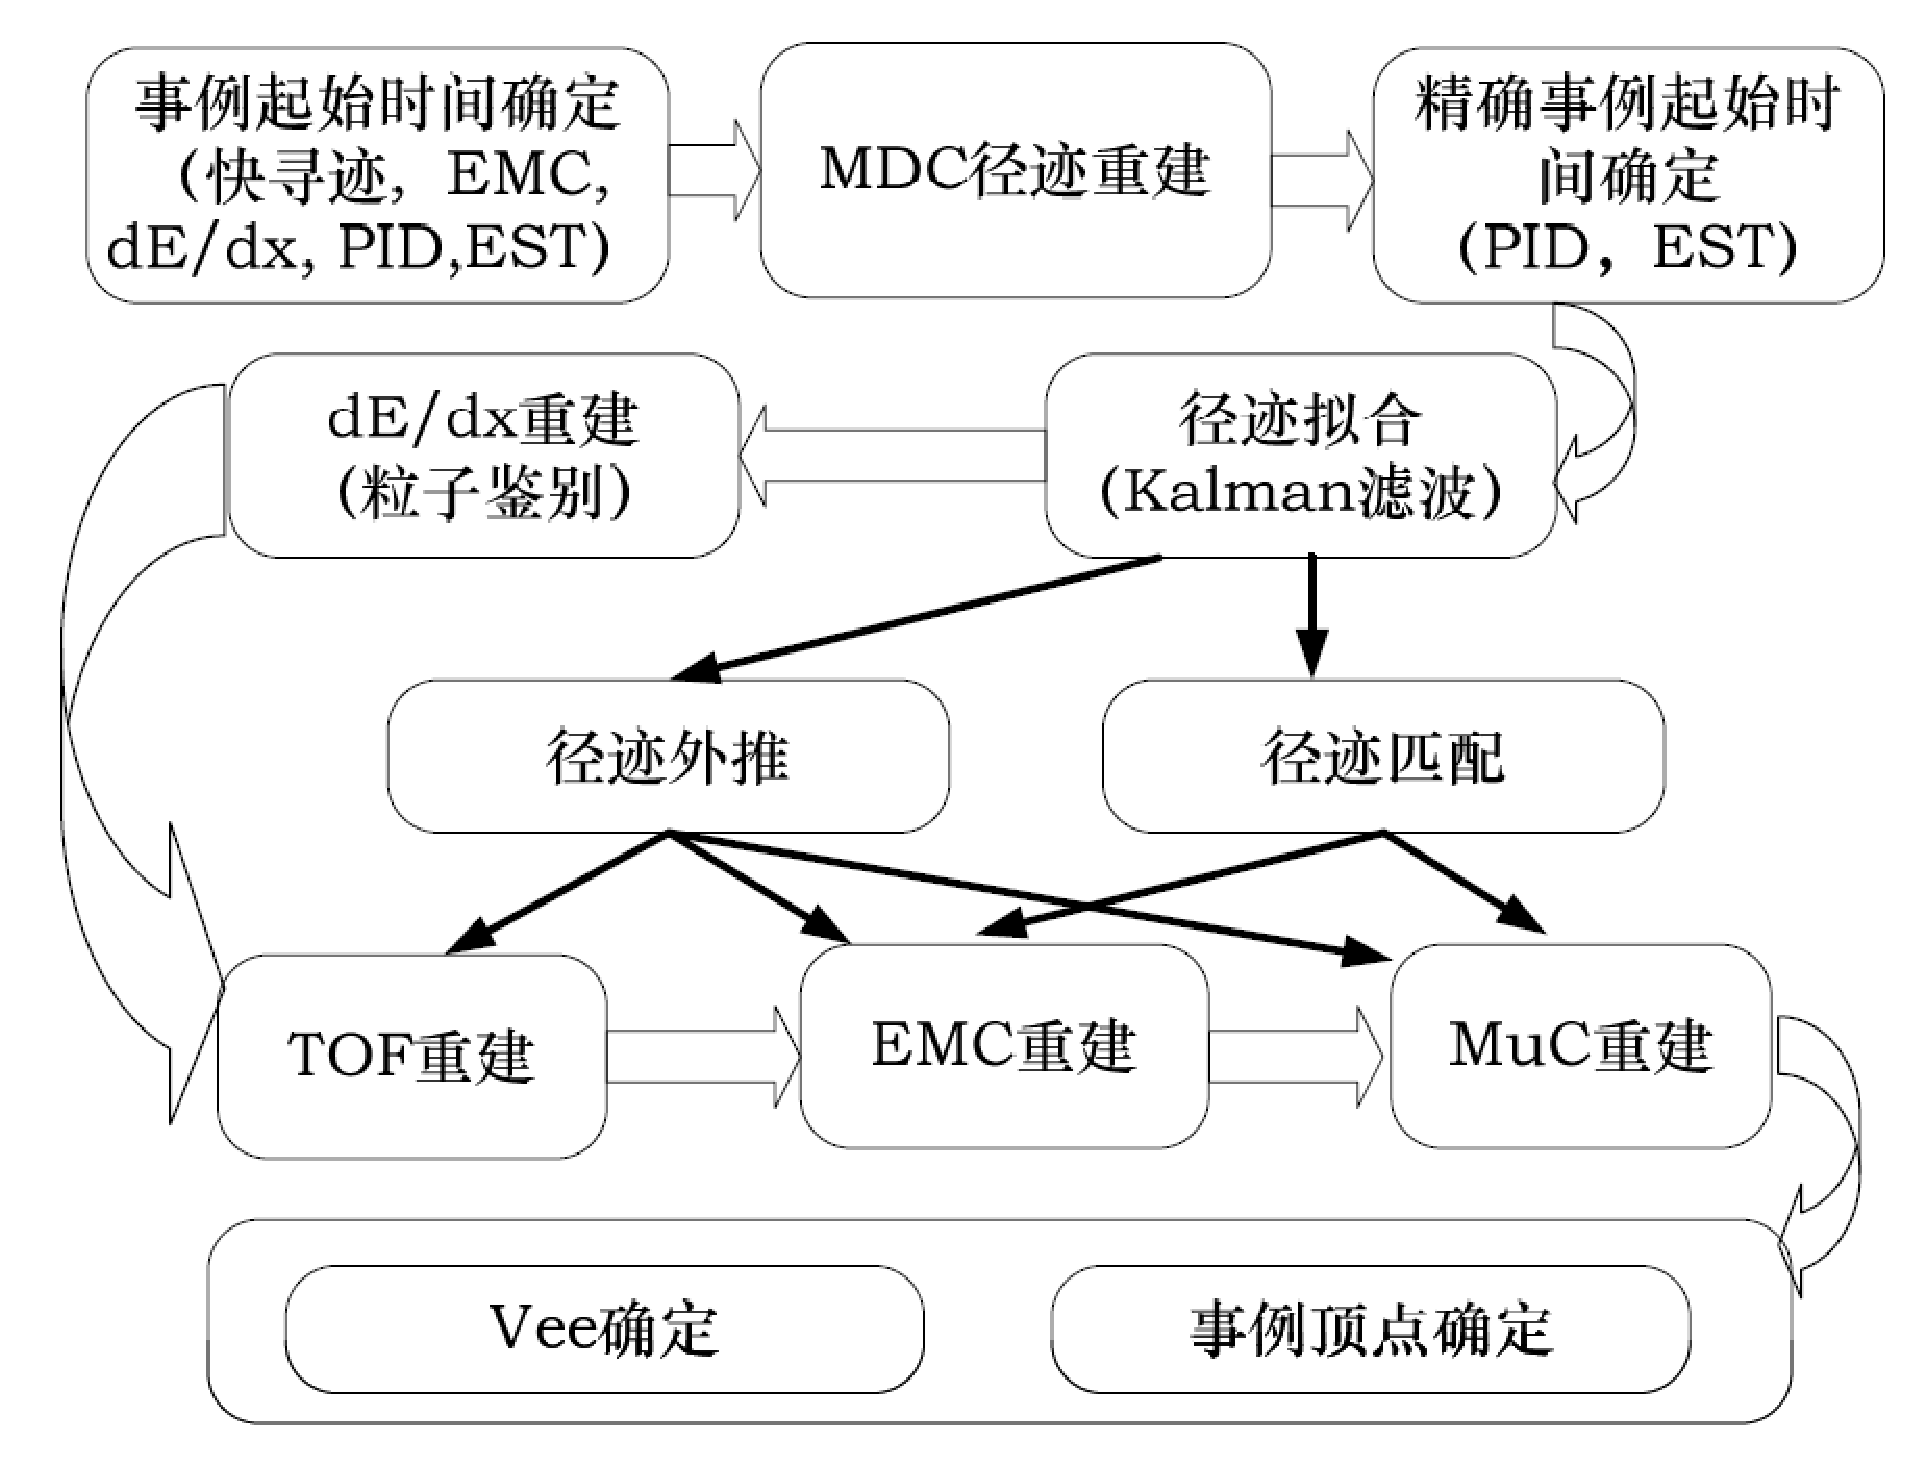
\includegraphics[width=0.65\textwidth]{bes3/rec_flow.eps}
 \caption{BESIII~的离线重建流程。}
 \label{fig:rec_flow}
 \end{center}
\end{figure}

\subsection{离线刻度系统}
正如前所述,末态粒子在各子探测器中留下的信息一般是以信号幅
度~(ADC)~和时间~(TDC)~的形式被记录下来的,但是各个子探测器
的工作状态并不是恒定不变的,同一子探测器的各部分相应也不一定均匀,
因入射粒子的角度不同探测器的响应也有所不同。因此必须有一套
能够精确反映各子探测器响应状态的参数,这套参数就是刻度常数。
离线刻度系统的任务就是获得这些刻度常数并对原始数据作系统的修正,
从而使测得的物理量更加准确。

\subsection{物理分析工具}
物理分析工具是一些为物理分析提供服务的公用的算法和接口。
BESIII~中的物理分析工具包括运动学拟合~(Kinematic Fitting)
~\cite{Yan:2010zze}、顶点拟合~(Vertex Fitting)、粒子鉴别~
(Particle Identification,PID)~\cite{Gang_2008}~和
事例组装~(Event Assembly)、亮度测量~(Luminosity Measurements)~
和分波分析~(Partial Wave Analysis,PWA)~等分析软件包。
这些软件能很好地提高物理分析的效率。

\section{本章小节}
本章介绍了BEPCII和BESIII的结构、BESIII 各个子系统的结构性能和共作原理等,
以及BESIII上的在线数据获取系统和离线软件系统。


